\section[Vymedzenie pojmov a úvod do problematiky]{Vymedzenie pojmov\\ úvod do problematiky}

  \emph{Senzor} je elektronické zariadenie, ktoré sníma okolie z~fyzikálneho hľadiska, pričom jeho výstupom sú digitálne spracovateľné údaje. Poskytuje priame vnímanie prostredia, v~ktorom je zasadený. Na zvýšenie kompletnosti a~presnosti informácií o~prostredí sa obvykle používa viacero snímačov súčasne~\cite{kolarSurveyDatafusionTechniques2020}. Pojmy \emph{senzor} a \emph{snímač} v tejto práci používame zameniteľne.
  
  \emph{Fúzia údajov} je proces zlučovania dát z~viacerých snímačov za účelom zníženia neistoty, ktorá vzniká pri navigácii a~pohybe vozidla prostredím~\cite{tzafestas12MobileRobot2014}. Fúzia pomáha vytvoriť presnejší model prostredia na spoľahlivejšie navigovanie a~správanie vozidla. 
  
  Inak povedané, fúzia dát zo snímačov je kombinácia senzorických dát alebo dát odvodených zo senzorických dát, pričom výsledná informácia je v~istom zmysle lepšia než by bola v~prípade použitia týchto zdrojov samostatne~\cite{elmenreichIntroductionSensorFusion}.

  Pojmy \emph{fúzia dát (zo snímačov)}, \emph{fúzia údajov (zo snímačov)}, \emph{fúzia snímačov}, apod.\ používame v tejto práci zameniteľne.

  \emph{Lokalizácia} označuje odhad polohy (pozície a orientácie) robota vzhľadom na referenčný súradnicový systém. Môže byť buď absolútna (vzhľadom na mapu prostredia) alebo relatívna (vzhľadom na predošlú polohu)~\cite{thrunProbabilisticRobotics2005}. V tejto práci budeme používať pojmy \emph{lokalizácia} a \emph{odhad/určenie polohy} zameniteľne.

  \subsection{Taxonómia fúzie}
      
    \noindent Podľa~\cite{tzafestas12MobileRobot2014} existujú tri základné typy viacsenzorovej architektúry:
    \begin{itemize}
        \item \emph{Redundantná}~--~všetky senzory poskytujú rovnaké informácie o~prostredí,
        \item \emph{Doplnková}~--~senzory poskytujú nezávislé typy informácií o~prostredí,
        \item \emph{Koordinovaná}~--~senzory zbierajú informácie o~prostredí sekvenčne.
    \end{itemize}
    Tri základné komunikačné schémy medzi senzormi sú~\cite{tzafestas12MobileRobot2014}:
    \begin{itemize}
        \item \emph{Decentralizovaná}~--~medzi uzlami senzorov neprebieha žiadna komunikácia,
        \item \emph{Centralizovaná}~--~všetky senzory poskytujú merania ústrednému uzlu,
        \item \emph{Distribuovaná}~--~uzly si vzájomne vymieňajú informácie danou frekvenciou (napr.\ každých 5 meraní, t.\ j.\ $\frac{1}{5}$ snímacej frekvencie).
    \end{itemize}
    Centralizovaná schéma sa dá považovať za špeciálny prípad distribuovanej, keď senzory spolu komunikujú po každom meraní.
    
    Fúziu údajov z~viacerých snímačov je možné vykonávať na rôznych úrovniach~\cite{elmenreichIntroductionSensorFusion}:
    \begin{itemize}
        \item \emph{Fúzia nízkej úrovne} (angl.\ \textit{low-level fusion, raw data fusion})~--~spočíva v~zlúčení surových dát z~viacerých zariadení za účelom produkovania nových dát obsahujúcich širšie spektrum informácií;
        
        \item \emph{Fúzia strednej úrovne} (angl.\ \textit{intermediate-level fusion, feature level fusion})~--~kombinuje rôzne príznaky, ako napríklad hrany, rohy, línie, textúry alebo pozície do mapy príznakov, ktorá môže byť následne využitá na segmentáciu a~detekciu;
        
        \item \emph{Fúzia vysokej úrovne} (angl.\ \textit{high-level fusion, decision fusion})~--~kombinuje rozhodnutia viacerých expertných algoritmov. Medzi používané metódy rozhodovania patria hlasovanie (angl.\ \textit{voting}), fuzzy logika či štatistické metódy.
    \end{itemize}
    
    Spoločným predpokladom na fúziu údajov z~viacerých snímačov je časová synchronizácia dát a~reprezentácia v~spoločnom súradnicovom systéme~\cite{laganiereSensorFusionAutonomous2021}.

  \subsection{Význam fúzie}
      
      Presnosť každého snímača je limitovaná určitými faktormi. Individuálne použitie akéhokoľvek snímača bez porovnania s~podobnými informáciami z~iných snímačov môže ovplyvniť celý systém, v~ktorom je implementovaný, pričom nie je možné odhaliť odchýlku alebo neplatnosť merania. Vo všeobecnosti sa pri senzorických meraniach môžeme stretnúť s~týmito nedostatkami~\cite{elmenreichIntroductionSensorFusion}:
      \begin{itemize}
          \item \emph{výpadok senzora}~--~porucha senzora spôsobuje stratu vnímania objektu,
          \item \emph{obmedzené pokrytie priestoru}~--~jediný senzor obvykle poskytuje informácie len z~určitého regiónu,
          \item \emph{obmedzené časové pokrytie}~--~na vykonanie merania a~sprenesenia informácie je potrebný určitý čas, čo limituje maximálnu frekvenciu meraní,
          \item \emph{nepresnosť}~--~merania sú limitované presnosťou snímača.
          \item \emph{neistota}~--~na rozdiel od nepresnosti závisí skôr od snímaného objektu než od snímača. Narastá keď senzor nedokáže zaznamenať všetky vlastnosti objektu alebo keď je meranie nejednoznačné. Systém s~jediným senzorom nedokáže znížiť neistotu vnímania kvôli obmedzenému pohľadu na objekt.
      \end{itemize}
          
      Naproti tomu, od fúzie dát zo snímačov si sľubujeme najmä tieto výhody~\cite{elmenreichIntroductionSensorFusion}:
      \begin{itemize}
          \item \emph{robustnosť a~spoľahlivosť}~--~pre systémy s~viacerými senzormi je prirodzená redundancia, ktorá umožňuje poskytovanie informácií aj v~prípade čiastočnej poruchy;
          \item \emph{rozšírené pokrytie priestoru a~času}~--~jeden senzor sa môže pozerať tam, kde (resp.\ v~čase, v~ktorom) iné nemôžu;
          \item \emph{zvýšenie presnosti a~opakovateľnosti}~--~meranie jedného senzora je porovnávané s~meraniami ostatných, snímajúcich tú istú veličinu;
          \item \emph{zníženie nejednoznačnosti a~neistoty}~--~zjednotené informácie znižujú množstvo nejednoznačných interpretácií meranej hodnoty;
          \item \emph{odolnosť voči rušeniu}~--~rozšírením dimenzie meraného priestoru sa systém stáva menej náchylným voči rušivým faktorom.
      \end{itemize}
          
      Keďže lokalizácia predstavuje kľúčovú úlohu v každom autonómne riadenom mobilnom systéme, je nevhodné sa pre jej odvodenie spoliehať len na jediný zdroj informácie. Nepresná lokalizácia totiž môže veľmi rýchlo viesť ku kumulácii chyby v mape prostredia a celkovej neschopnosti robota orientovať sa v prostredí. Metóda fúzie údajov z viacerých snímačov musí zohľadňovať ich chybové či meracie vlastnosti. Prehľad dôležitých parametrov, ktoré definujú vlastnosti snímačov, ako aj ich zatriedenie podľa rôznych kritérií prinášame v nasledujúcej kapitole. V~neposlednom rade, zo softvérového hľadiska slúži fúzia ako rozhranie pre nasledujúce úlohy, tie sa tak stávajú nezávislé od zdroja meraní.

\subsection{Vlastnosti a~taxonómia snímačov}

Pokiaľ je našou snahou fúzia senzorických dát, musíme v prvom rade poznať parametre týchto senzorov, ich silné a slabé stránky, pretože to sú faktory, ktoré je pri fúzii potrebné zohľadniť.  

V~súvislosti so snímačmi používanými v~mobilnej robotike treba mať na pamäti tri zásadné skutočnosti~\cite{duchonSnimaceMobilnejRobotike2012}:
  \begin{enumerate}
    \item Meranie skutočnými snímačmi je zašumené;
    \item Skutočné snímače poskytujú nekompletný opis prostredia;
    \item Skutočné snímače nemôžu byť úplne modelované.
  \end{enumerate}

  \begin{figure}[t!]
    \centering
    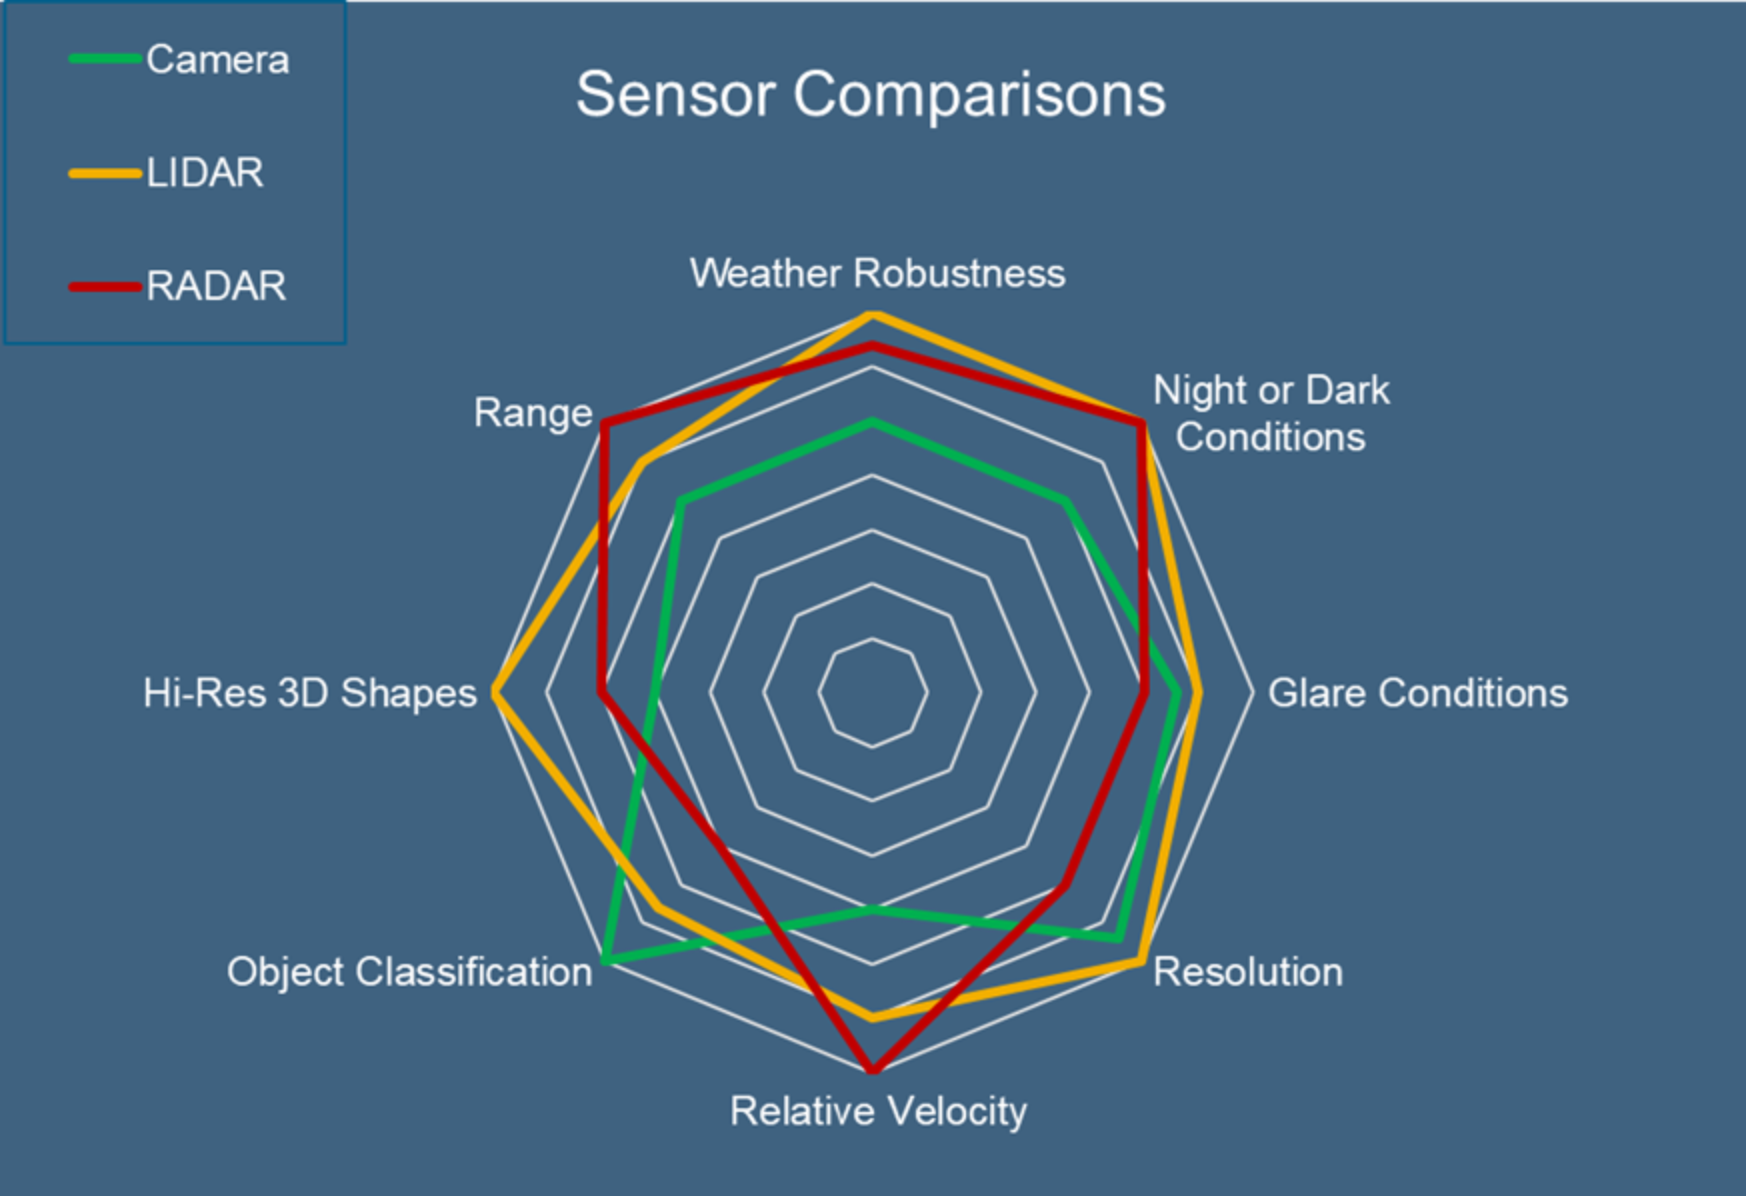
\includegraphics[width=\textwidth]{img/sensor_comparision.png}
    \caption[Diagram porovnania vybraných snímačov podľa vlastností]{Diagram porovnania vybraných snímačov podľa dosahu, rozlíšenia, schopnosti klasifikácie, určovania rýchlosti a odolnosti pri rôznych vonkajších podmienkach~\cite{WhySensorFusion2024}.}\label{fig:sensor-comparision}
  \end{figure}


  Vlastnosti a~miera použiteľnosti snímačov sú dané mnohými parametrami, ktoré ich vzájomne odlišujú. Porovnanie vlastností vybraných typov snímačov je znázornené na obr.~\ref{fig:sensor-comparision}. Medzi najvýznamnejšie parametre snímačov môžeme zaradiť~\cite{duchonSnimaceMobilnejRobotike2012}:
  \begin{itemize}
    \item \emph{Zorné (detekčné) pole (\acrshort{fov})}~--~šírka záberu snímača, zvyčajne vyjadrená v~stupňoch. Niektoré typy snímačov majú definované vertikálne aj horizontálne zorné pole;
    \item \emph{Merací rozsah}~--~pracovný rozsah snímania vrátane obmedzenia hĺbky (môže byť minimálne aj maximálne);
    \item \emph{Dynamický rozsah}~--~pomer medzi maximálnou a~minimálnou vstupnou hodnotou snímača. Hodnota býva vyjadrená v~decibeloch;
    \item \emph{Rozlíšenie}~--~minimálny rozdiel medzi dvoma hodnotami, ktoré snímač dokáže detegovať;
    \item \emph{Lineárnosť}~--~ak je gradient vstupno-výstupnej závislosti konštantný, snímač je lineárny;
    \item \emph{Šírka pásma/frekvencia}~--~rýchlosť merania snímača. Zvyčajne býva vyjadrená v~hertzoch;
    \item \emph{Citlivosť}~--~miera zmeny výstupného signálu vzhľadom na mieru zmeny vstupného signálu. Môže byť ovplyvnená aj prostredím;
    \item \emph{Chyba}~--~odchýlka výstupnej hodnoty od skutočnej. Vo všeobecnosti rozlišujeme medzi dvomi typmi chýb:
    \begin{itemize}
      \item \emph{systematická (deterministická)}~--~sústavná (konštantná) odchýlka meraní od skutočnosti. Môže byť spôsobená faktormi alebo procesmi, ktoré je možné modelovať;
      \item \emph{náhodná (stochastická)}~--~premenlivá odchýlka meraní od skutočnosti. Je možné ju vyjadriť pravdepodobnostnými metrikami;
    \end{itemize}
    \item \emph{Presnosť}~--~miera systematickej chyby. Vyjadrená býva v~pomere k~skutočnej hodnote;
    \item \emph{Opakovateľnosť}~--~miera náhodnej chyby. Je nezávislá od presnosti snímača;
    \item \emph{Drift}~--~postupný odklon meraní od reálnych hodnôt, vzniká kumuláciou chýb merania;
    \item \emph{Latencia}~--~oneskorenie medzi momentom výskytu fyzikálneho javu a~momentom poskytnutia informácie o~ňom senzorom. Môže byť spôsobená viacerými faktormi, vrátane fyzikálnych vlastností senzora, spôsobu spracovania signálu či času potrebného na odoslanie údajov.
  \end{itemize}

  Snímače a~systémové komponenty využívané na lokalizáciu mobilných robotov možno klasifikovať viacerými spôsobmi podľa rôznych hľadísk, vo všeobecnosti podľa toho čo a~akým spôsobom snímajú. Každé z~týchto hľadísk zvýrazňuje iný aspekt senzorov. Medzi najčastejšie kritériá taxonómie snímačov patria:

\begin{enumerate}
  \item Podľa spôsobu interakcie so snímaným prostredím~\cite{christensenSensingEstimation2016}:
  \begin{itemize}
    \item \emph{Aktívne}~--~senzory, ktoré samy vysielajú energiu do prostredia (napr.\ \acrshort{lidar}, ultrazvuk),
    \item \emph{Pasívne}~--~senzory, ktoré len pasívne prijímajú signály (napr.\ kamery, magnetometre),
  \end{itemize}

  \item Podľa typu meranej veličiny~\autocite{siegwartIntroductionAutonomousMobile2011,thrunProbabilisticRobotics2005}:
  \begin{itemize}
    \item \emph{inerciálne veličiny}~--~gyroskopy, akcelerometre,
    \item \emph{vzdialenosť}~--~\acrshort{lidar}, ultrazvuk,
    \item \emph{elektromagnetické signály}~--~\acrshort{gnss}, magnetometre;
  \end{itemize}
  
  \item Podľa referenčného rámca výstupu~\cite{inproceedings}:
  \begin{itemize}
    \item \emph{Lokálne}~--~poskytujú odhad polohy vzhľadom na predchádzajúci stav robota (napr.\ odometria),
    \item \emph{Globálne}~--~poskytujú polohu vzhľadom na externý (globálny) rámec (napr.\ GNSS, \acrshort{mocap} systémy);
  \end{itemize}
  
  \item Podľa spôsobu vnímania~\cite{siegwartIntroductionAutonomousMobile2011}:
  \begin{itemize}
    \item \emph{Proprioreceptívne}~--~merajú vnútorný stav robota samotného (napr.\ \acrshort{imu}),
    \item \emph{Exteroreceptívne}~--~merajú informácie o~vonkajšom prostredí (napr.\ \acrshort{lidar}, kamera);
  \end{itemize}
  
  \item Podľa požiadaviek na infraštruktúru~\cite{ferreiraVehicleLocalizationSystem2013}:
  \begin{itemize}
    \item \emph{Interné (\uv{on-board})}~--~schopné fungovať samostatne ako súčasť robota, bez potreby externej infraštruktúry (napr.\ kamera, \acrshort{lidar}, \acrshort{imu}),
    \item \emph{Externé (\uv{off-board})}~--~vyžadujú vopred pripravené externé prvky poskytujúce referenčné informácie (napr.\ \acrshort{gps}, \acrshort{mocap}, \acrshort{uwb});
  \end{itemize}
  \end{enumerate}

  Pri návrhu senzorického vybavenia pre lokalizáciu mobilného robota je potrebné vychádzať z~možností, ktoré poskytuje daná aplikácia. Pred voľbou konkrétnych snímačov si musí dizajnér položiť niekoľko rozhodujúcich otázok. Bude sa robot pohybovať v~exteriéri alebo interiéri? Ak v~interiéri, pôjde o~vopred známe prostredie s~možnosťou prispôsobenia infraštruktúry, alebo to bude neznáme prostredie, v~ktorom musí byť robot schopný operovať s~vlastnou výbavou? Ak v~exteriéri, bude sa robot pohybovať v~prostrediach s~dobrým pokrytím \acrshort{gnss}, alebo skôr v~lesnatých či zastavaných oblastiach? Akú časť z~celkovej hmotnosti robota je možné rezervovať pre senzory pri zohľadnení dynamických požiadaviek aplikácie? S~akým rizikom kolízie či poškodenia robota sa pri danej aplikácii počíta a~akú časť celkovej ceny robota môžu tvoriť práve senzory?

  Odpovede na tieto otázky je možné premietnuť na jednu škálu ohraničenú práve voľbou medzi použitím interných alebo externých senzorov. V~tejto práci sa preto na systematizáciu predstavenia senzorov používaných na lokalizáciu mobilných robotov použijeme práve poslednú spomenutú taxonómiu.